\documentclass{article}

\usepackage{xurl}
\usepackage{hyperref}
\usepackage{graphicx}
\usepackage{listings}

\title{
\includegraphics[width=\textwidth]{images/cover.jpg}\\Measuring Software Engineering}
\author{Lexes Jan Mantiquilla}
\date{\today}

\begin{document}

\maketitle
\newpage

\tableofcontents
\newpage

\section{Introduction}
This report will focus on explaining the various ways in which one can measure
the software engineering process. The report outline what platforms or
frameworks are available to perform measurement. As well as that, the report
will go through the algorithmic approaches and the ethic concerns surrounding
the measurement of the software engineering process.

\section{Why measure software engineering}
There are many benefits to measuring software engineering. Most notably to
produce higher quality code, to reduce the cost of software development and to
improve the speed at which software development takes place.
\subsection{More specifically, measuring software engineering:}
\begin{itemize}
  \item Helps in identifying possible software defects early in development
  \item Increase the work load that the current staff can accomplish
  \item Identify high-output employees to receive rewards and low-output
    employees to receive help and training.
  \item Increase the complexity and value of the software with the same staff
    effort.
\end{itemize}
~\cite{scacchi1995understanding}

It is clear that measuring software engineering has many benefits. Thus, many
companies strive to create and or use services which perform such measurement.
However, there are some ethical concerns and inefficient methods of measuring
software engineering which will be explored further in the next section.

\section{How software engineering can be measured}
There are many individual metrics which can be measured during the development
of software which may indicate progress. Most of software engineering is
measured using a version control system. Version control systems generate vast
amounts of data which can then be measured. The main metrics that this report
will go through are lines of code, number of pull requests and code review
turnaround time.

\subsection{Lines of code}
The most simplest metric to measure would be the lines of code (LOC). LOC is a
simple and crude method to measure the productivity of a software engineer.
Using LOC rewards bad coding practices and less efficient
code.~\cite{fenton1999software} This is evident in the short Java code example
below.

\subsubsection{Version 1}
\begin{lstlisting}[language=Java,frame=single,firstnumber=0,numbers=left,label={lst:v1}]
for (int i = 0; i < 5; i++) {
  System.out.println("Hello world");
}
\end{lstlisting}

\subsubsection{Version 2}
\begin{lstlisting}[language=Java,frame=single,firstnumber=0,numbers=left,label={lst:v2}]
System.out.println("Hello world");
System.out.println("Hello world");
System.out.println("Hello world");
System.out.println("Hello world");
System.out.println("Hello world");
\end{lstlisting}

The versions~\ref{lst:v1} and~\ref{lst:v2} of the code produce the same output.
However it is clear which version of the code is more desirable. The
version~\ref{lst:v1} of the code is follows good coding practices. It is DRY
(don't repeat yourself). The version~\ref{lst:v2} on the other hand is bad
quality code compared to the first version.

Other reasons why using LOC as a metric to measure productivity is not a good
idea is that it does not take into account formatting. It is also not language
agnostic. This is seen in the examples below.

\subsubsection{Version 1}
\begin{lstlisting}[language=Java,frame=single,firstnumber=0,numbers=left,label={lst:fmtv1}]
if (i < 2) {
  i++;
} else if (i > 10) {
  i--;
}
\end{lstlisting}

\subsubsection{Version 2}
\begin{lstlisting}[language=Java,frame=single,firstnumber=0,numbers=left,label={lst:fmtv2}]
if (i < 2) { i++; } else if (i > 10) { i--; }
\end{lstlisting}

\subsubsection{Version 3}
\begin{lstlisting}[language={[x86masm]Assembler},frame=single,firstnumber=0,numbers=left,label={lst:fmtv3}]
  cmp rcx, #2
  jge ifIge2
  inc rcx
  jmp eIf
ifIge2:
  cmp rcx, #10
  jle eIf
  dec rcx
eIf
\end{lstlisting}

Yet again all three versions of the code is equivalent however it is not clear
from the LOC which software engineer is more productive.

\subsection{Number of pull requests}
The general idea is that the more pull requests completed, the more productive
a team is. This method however does not measure productivity well. Like
counting lines of code, using the number of pull requests created also favors
bad programming practices. It encourages small and unnecessary pull requests.
The size and the difficulty of the pull request is also not taken into account.

\begin{figure}[h]
  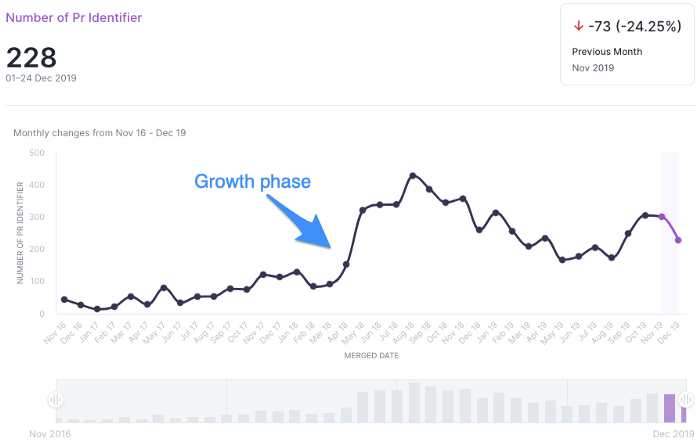
\includegraphics[width=\linewidth]{images/number_of_pr.png}
  \caption{Example number of pull requests metric, courtesy of
  Medium~\cite{metrics2020wrong}}
\end{figure}

\subsection{Code review turnaround time}
A more modern approach to measuring software engineer productivity would be to
measure process metrics instead of product metrics. Some examples of product
metrics would be the lines of code or the number of commits / pull requests
completed.

The code review turnaround time is an example of process metrics. Whenever code
is added or changed in a code base, it must undergo a code review process. This
usually involves other coworkers looking over code and making suggestions
before the code can be merged into the main branch. The general idea is to
measure how long it takes until a code review is done.

According to Abi Noda measuring process metrics is a great way to increase
productivity. Process metrics directly impact the developer experience in a
positive way. Not only that, but it is also a great way to show how the
organization is improving.~\cite{elusive2019quest}

\section{Platforms available}
Measuring the software engineering process is a valuable process. Thus, many
services have been created to aid companies analyze and display this process.
The data provided by the services help employers visualize whether or not the
ongoing projects will be delivered on time, see which employees have a high
impact on the company, etc.

\subsection{Pluralsight Flow}
Pluralsight Flow, called GitPrime previously, is a service which obtains data
from git host, e.g. GitHub, and the git information from repositories which the
engineers work on.~\cite{plural2019sight} The said data is processed to produce
useful metrics to indicate the performance of software engineers.

Version Control Systems like git generate a large digital footprint for the
developers that use it. Information like the number of commits done by a
developer, the lines of code changed by a developer, is produced through the
use of a version control system. These metrics alone may not be a good
indication of the productivity of a software engineer. However, when processed
together, a clearer picture is obtained.

Pluralsight Flow, for example, will use the information found pull requests
(PRs), tickets linked to said PRs and commits to produce useful graphs and
metrics.

\subsubsection{New metrics extrapolated by Pluralsight Flow:}
\begin{itemize}
  \item Churn --- The amount of code which is changed or deleted shortly after
    it was written. A high amount of churn may indicate that something may be
    affecting the development life cycle.
  \item Efficiency --- A percentage evaluating whether the committed code is
    productive work. This metric is directly related to the churn metric.
  \item Impact --- A score given to a commit which measures the effect of
    changing or adding specific lines of code. This metric uses many factors to
    determine the score such as the amount of code changed, the number of files
    affected, the percentage of old code edited and many more.
\end{itemize}
~\cite{plural2019sight2}

\subsection{Azure DevOps services}
Azure DevOps services is a collection of developer services provided by
Microsoft to facilitate the software engineering process. There are many Azure
DevOps services available however this report focus on the Azure Boards and the
Azure Pipelines service in particular.~\cite{azure2020devops}

\subsubsection{Azure Boards}
Azure Boards is a service which allows software engineers to track and manage
their work for software projects. Azure Boards is built with software
engineering processes in mind and has native support for Kanban and Scrum. It
offers built-in scrum boards and and tools to help the team run sprints and
stand-ups.

The basis of Azure Boards is an entity called the `work item'. This entity
tracks all the work done for the software project. A `work item' communicates
the details of the work to be completed to the team. Each `work item' has a
status attached which is an indication the progress of the work. This allows
the whole team to be on the same page with regards to what work is assigned to
who and whether or not it has been completed.

Each `work item' has a rich set of information attached to it. It contains
information such as links to discussions regarding the `work item', any
commits, PRs or tickets related, as well as a history of all changes to the
`work item'.

The information collected through the use of Azure Boards is analyzed and
presented on a dashboard which indicates the health of the project. The
dashboard contains all the metrics gathered, such as the velocity of the
project or average completion time, in one place.~\cite{azure2020boards}

\subsubsection{Azure Pipelines}
Azure Pipelines is a cloud continuous integration (CI) and continuous delivery
(CD) service. That is, a service which builds, tests and deploys your code
automatically. This service is used in conjunction with a git host such as
GitHub or Azure Repos.

The metrics which Azure Pipelines provides are the pipeline pass rate, the code
test pass rate and the average pipeline duration. The information for the
pipeline analytics is obtained from the pipeline runs.

\section{Algorithmic approaches}

\subsection{COCOMO}
COCOMO (Constructive Cost Model) is a regression model which is used to
estimate the cost, effort and the development time to produce a software
project. This model was produced by Barry W. Boehm~\cite{barry1981software}.

Software projects which use the COCOMO model are classified into three
categories which are organic, semi-detached and embedded. The definition of
each is found in figure~\ref{fig:catagories} below.

\begin{figure}[h]
  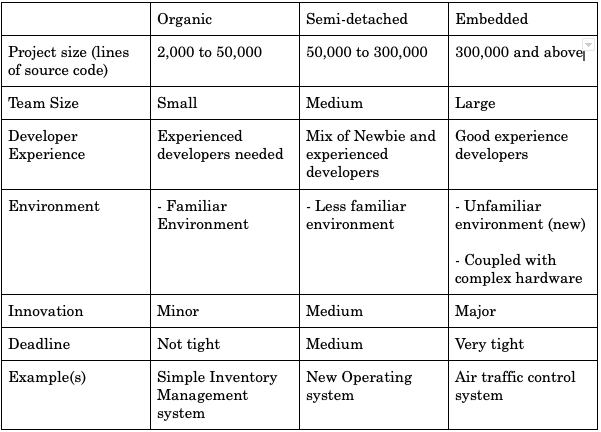
\includegraphics[width=\linewidth]{images/cocomo_categories.png}
  \caption{\raggedright{}Definition of the different COCOMO categories,
  courtesy of Medium~\cite{cocomo2020procedural}}\label{fig:catagories}
\end{figure}

The different categories influence the algorithms used during the calculation
of the estimates.

The COCOMO model has three different types which allow the software manager to
specify the granularity of the estimates.

\subsubsection*{The different types are:}
\begin{itemize}
  \item Basic COCOMO model --- This model is quite limited and restricted as it
    uses kilo lines of code for the calculations. This model does not take into
    account the other factors for the estimations.
  \item Intermediate COCOMO model --- This model builds on top of the basic
    COCOMO model and takes cost drivers into account which further enhances the
    estimate. A cost driver is a term used to define factors which have an
    effect on the effort, cost and time during the development phase of a
    software project.
  \item Detailed COCOMO model --- Yet again this model builds on top of the
    basic and intermediate model and incorporates the Waterfall model e.g.\ the
    the cost estimates are completed at every step of the waterfall model. This
    is the most accurate model available in the COCOMO models.
\end{itemize}

\subsection{Machine learning}
``Machine learning is the study of computer algorithms that allow computer
programs to automatically improve through
experience.~\cite{machine1997learning}'' Nowadays machine learning is used
extensively. They power things from self-driving cars to spam filtering. The
applications of machine learning are endless.

In order to use machine learning, one must have a large data set to work with.
One of the side effects of using a version control system is that it produces a
large data set regarding software engineering. One application of machine
learning is to process the data from version control systems to measure
software development productivity.

Firstly, we must define what it means to be a productive software engineer. A
highly productive software engineer is one which produces more source code and
source code of a higher quality. Through the use of machine learning
techniques, the complex code structure produced by software engineers is
reduced into quantitative measures of quality and
quantity.~\cite{helie2018measuring}

\section{Ethics}

\section{Conclusion}

\newpage

\bibliographystyle{plain}
\bibliography{bibliography.bib}

\end{document}
